\documentclass[10pt,letterpaper]{article}

\usepackage[T1]{fontenc}
\usepackage[utf8]{inputenc}
\usepackage{helvet}
\renewcommand{\familydefault}{\sfdefault}

\usepackage[left=17mm,right=17mm,top=20mm,bottom=22mm,headheight=20pt]{geometry}
\usepackage{amsmath,amssymb}
\usepackage[table]{xcolor}
\usepackage{graphicx}
\usepackage{booktabs}
\usepackage{tabularx}
\usepackage{array}
\usepackage{fancyhdr}
\usepackage{enumitem}
\usepackage{tcolorbox}
\tcbuselibrary{most}
\usepackage{pgfplots}
\pgfplotsset{compat=1.18}
\usepgfplotslibrary{fillbetween}
\usetikzlibrary{positioning,calc,shapes.geometric,decorations.pathmorphing,backgrounds,patterns}
\usepackage{fontawesome5}
\usepackage{lastpage}
\usepackage[colorlinks=true,linkcolor=ptteal,urlcolor=ptteal]{hyperref}

\definecolor{ptteal}{HTML}{0E5C63}
\definecolor{ptamber}{HTML}{C9852E}
\definecolor{ptslate}{HTML}{32404C}
\definecolor{ptbg}{HTML}{F2F6F5}
\definecolor{ptgreen}{HTML}{4C7A50}
\definecolor{ptred}{HTML}{A63A3A}

\setlength{\parindent}{0pt}
\setlength{\parskip}{2pt}

\pagestyle{fancy}
\fancyhf{}
\renewcommand{\headrulewidth}{0.6pt}
\renewcommand{\footrulewidth}{0.6pt}
\fancyheadoffset{0pt}
\renewcommand{\headrule}{\hbox to\headwidth{\color{ptteal}\leaders\hrule height \headrulewidth\hfill}}
\renewcommand{\footrule}{\hbox to\headwidth{\color{ptteal}\leaders\hrule height \footrulewidth\hfill}}
\fancyhead[L]{\color{ptslate}\sffamily\small\bfseries Meridian Rehabilitation \& Sports Medicine}
\fancyhead[R]{\color{ptslate}\sffamily\small Physical Therapy Progress Evaluation}
\fancyfoot[L]{\color{ptslate}\sffamily\footnotesize CONFIDENTIAL --- Protected Health Information}
\fancyfoot[R]{\color{ptslate}\sffamily\footnotesize Page \thepage\ of \pageref{LastPage}}

\newcommand{\sectiontitle}[2]{%
  \vspace{6pt}
  \noindent
  \begin{tikzpicture}
    \node[fill=ptteal,text=white,minimum height=0.62cm,inner sep=5pt,anchor=west] (icon) at (0,0) {\small #1};
    \node[fill=ptbg,text=ptslate,minimum height=0.62cm,inner sep=6pt,anchor=west,font=\bfseries\sffamily,minimum width=\dimexpr\linewidth-1.05cm\relax] (lbl) at (icon.east) {#2};
  \end{tikzpicture}
  \vspace{3pt}
}

\newcommand{\infoicon}[2]{\textcolor{ptteal}{#1}~#2}

\tcbset{goalbox/.style={colback=ptbg,colframe=ptteal,boxrule=0.6pt,arc=1.5pt,
    fonttitle=\bfseries\sffamily\small,coltitle=white,
    colbacktitle=ptteal,left=6pt,right=6pt,top=3pt,bottom=3pt}}

\newcommand{\metgoal}{\textcolor{ptgreen}{\faCheckCircle}}
\newcommand{\opengoal}{$\square$}

\title{Physical Therapy Progress Evaluation}
\author{Meridian Rehabilitation \& Sports Medicine}
\date{}

\begin{document}
\thispagestyle{fancy}

% ------------------------------------------------------------------
% TITLE BLOCK
% ------------------------------------------------------------------
\begin{center}
{\Large\bfseries\sffamily\color{ptteal} Meridian Rehabilitation \& Sports Medicine}\\[2pt]
{\small\color{ptslate} Apex Campus Outpatient Orthopedic \& Sports Rehabilitation Center}\\[1pt]
{\footnotesize\color{ptslate}
  \infoicon{\faMapMarker}{2140 Fenwick Boulevard, Suite 310, Cedar Hollow, OH 44311} \quad
  \infoicon{\faPhone}{(330) 555-0148} \quad
  \infoicon{\faFile}{(330) 555-0149 (fax)}
}
\end{center}

\vspace{4pt}
\noindent\rule{\linewidth}{1.4pt}
\vspace{2pt}

\begin{center}
{\LARGE\bfseries\sffamily\color{ptslate} Physical Therapy Progress Evaluation}\\[2pt]
{\small\sffamily\color{ptamber}\bfseries Re-Evaluation --- Visit 12 of 24 Authorized}
\end{center}
\vspace{6pt}

% ------------------------------------------------------------------
% PATIENT / CASE INFORMATION
% ------------------------------------------------------------------
\sectiontitle{\faUser}{Patient \& Case Information}

\begin{tabularx}{\linewidth}{@{}>{\bfseries\raggedright\arraybackslash}p{3.4cm} X >{\bfseries\raggedright\arraybackslash}p{3.4cm} X@{}}
\toprule
Patient Name & Marcus J.\ Delgado & Date of Birth & March 14, 1979 (Age 47) \\
Medical Record \# & MRN-885204 & Sex & Male \\
Referring Physician & Dr.\ Elena Whitfield, MD --- Apex Orthopedic Group & Date of Surgery & May 4, 2026 \\
Diagnosis & S/P Right Total Knee Arthroplasty (TKA) & ICD-10 Code & Z47.1, M17.11 \\
Initial Evaluation & May 6, 2026 & Progress Evaluation Date & June 30, 2026 (Week 8) \\
Treating Therapist & Rachel Nakamura, PT, DPT, OCS & Visit Frequency & 3x/week, 8 weeks \\
Insurance Payer & Vertex Health Partners --- PPO & Authorization \# & VHP-2026-0453 (24 visits) \\
\bottomrule
\end{tabularx}

\vspace{4pt}
\begin{tcolorbox}[colback=ptbg,colframe=ptteal!70,boxrule=0.5pt,arc=1.5pt,left=6pt,right=6pt,top=3pt,bottom=3pt]
\small\textbf{Precautions:} Weight-bearing as tolerated with single-point cane for community distances $>$150m. No pivoting or deep squatting past 90$^\circ$ flexion under load until Week 10 per surgeon protocol. Patient is anticoagulated (apixaban) --- monitor for bruising and report any calf swelling asymmetry immediately.
\end{tcolorbox}

% ------------------------------------------------------------------
% SUBJECTIVE
% ------------------------------------------------------------------
\sectiontitle{\faPen}{Subjective}

Mr.\ Delgado presents for his scheduled eight-week progress evaluation following right total knee arthroplasty. He reports steady improvement in mobility and a marked reduction in resting pain since the initial evaluation. He has returned to part-time duties at his logistics coordinator role, seated for most of the shift with scheduled standing breaks, and ambulates the office corridor without an assistive device on level surfaces. His chief remaining complaints are stiffness after prolonged sitting and residual weakness when descending stairs.

\begin{itemize}[leftmargin=16pt,itemsep=1pt,topsep=2pt]
  \item \textbf{Pain (NPRS 0--10):} At rest 1/10 (initial: 4/10); with stair descent 4/10 (initial: 8/10); end-of-day 2/10 (initial: 6/10).
  \item \textbf{Sleep:} No longer waking due to knee pain; previously waking 2--3 times nightly at initial evaluation.
  \item \textbf{Function:} Independent with all bed mobility and transfers. Reports difficulty kneeling and squatting to retrieve items from low shelving.
  \item \textbf{Medication:} Weaned off scheduled opioid analgesia at Week 5; uses acetaminophen 500\,mg PRN, averaging fewer than two doses per week.
  \item \textbf{Patient goal:} Return to recreational doubles tennis and unrestricted travel (car and air) by Week 16.
\end{itemize}

% ------------------------------------------------------------------
% OBJECTIVE -- ROM
% ------------------------------------------------------------------
\sectiontitle{\faStethoscope}{Objective Findings}

\textbf{\color{ptslate}Range of Motion (Active, Goniometric, degrees)}

\begin{tabularx}{\linewidth}{@{}Xcccccc@{}}
\toprule
\textbf{Joint / Motion} & \textbf{Normal} & \textbf{Initial (Wk 0)} & \textbf{Prior (Wk 4)} & \textbf{Current (Wk 8)} & \textbf{Change} & \textbf{Goal} \\
\midrule
Right knee flexion & 0--135$^\circ$ & 68$^\circ$ & 95$^\circ$ & 115$^\circ$ & \textcolor{ptgreen}{+47$^\circ$} & 125$^\circ$ \\
Right knee extension & 0$^\circ$ & $-$12$^\circ$ & $-$5$^\circ$ & 0$^\circ$ & \textcolor{ptgreen}{+12$^\circ$} & 0$^\circ$ \\
Left knee flexion (uninvolved) & 0--135$^\circ$ & 132$^\circ$ & 133$^\circ$ & 134$^\circ$ & \textcolor{ptgreen}{+2$^\circ$} & 135$^\circ$ \\
Right hip flexion & 0--120$^\circ$ & 96$^\circ$ & 108$^\circ$ & 116$^\circ$ & \textcolor{ptgreen}{+20$^\circ$} & 120$^\circ$ \\
Right ankle dorsiflexion & 0--20$^\circ$ & 8$^\circ$ & 12$^\circ$ & 15$^\circ$ & \textcolor{ptgreen}{+7$^\circ$} & 18$^\circ$ \\
\bottomrule
\end{tabularx}

\vspace{6pt}
\textbf{\color{ptslate}Manual Muscle Testing (MMT, 0--5 Kendall Scale)}

\begin{tabularx}{\linewidth}{@{}X cc cc@{}}
\toprule
& \multicolumn{2}{c}{\textbf{Right (Involved)}} & \multicolumn{2}{c}{\textbf{Left (Uninvolved)}} \\
\cmidrule(lr){2-3}\cmidrule(lr){4-5}
\textbf{Muscle Group} & \textbf{Initial} & \textbf{Current} & \textbf{Initial} & \textbf{Current} \\
\midrule
Quadriceps & 2/5 & \cellcolor{ptgreen!15}4-/5 & 5/5 & 5/5 \\
Hamstrings & 3/5 & \cellcolor{ptgreen!15}4/5 & 5/5 & 5/5 \\
Hip abductors (gluteus medius) & 2+/5 & \cellcolor{ptgreen!15}4-/5 & 4+/5 & 5/5 \\
Hip flexors (iliopsoas) & 3/5 & \cellcolor{ptgreen!15}4/5 & 5/5 & 5/5 \\
Gastrocnemius/soleus & 3-/5 & \cellcolor{ptgreen!15}4/5 & 5/5 & 5/5 \\
Tibialis anterior & 3/5 & 4/5 & 5/5 & 5/5 \\
\bottomrule
\end{tabularx}
\vspace{2pt}
{\footnotesize\color{ptslate}\textit{Grading key: 0 = no contraction, 1 = trace, 2 = active movement gravity-eliminated, 3 = active movement against gravity, 4 = movement against moderate resistance, 5 = normal.}}

\vspace{6pt}
\textbf{\color{ptslate}Girth Measurements \& Effusion}

\begin{tabularx}{\linewidth}{@{}Xcccc@{}}
\toprule
\textbf{Location (Right knee)} & \textbf{Initial (cm)} & \textbf{Current (cm)} & \textbf{Left (cm)} & \textbf{Difference} \\
\midrule
Mid-patella & 42.5 & 39.0 & 38.5 & \textcolor{ptgreen}{$-$3.5} \\
15\,cm above joint line & 46.0 & 44.5 & 44.0 & \textcolor{ptgreen}{$-$1.5} \\
10\,cm below joint line & 34.5 & 33.0 & 32.5 & \textcolor{ptgreen}{$-$1.5} \\
\bottomrule
\end{tabularx}
\par\vspace{2pt}
{\footnotesize\color{ptslate}Trace effusion present with a negative sweep test, improved from moderate effusion (2+/4) at initial evaluation. Surgical incision well healed, no signs of infection.}

\vspace{4pt}
% ------------------------------------------------------------------
% GAIT / FUNCTIONAL MOBILITY
% ------------------------------------------------------------------
\textbf{\color{ptslate}Functional Mobility \& Gait}

\begin{itemize}[leftmargin=16pt,itemsep=1pt,topsep=2pt]
  \item \textbf{Assistive device:} Single-point cane, left hand, for community ambulation $>$150m; none required indoors.
  \item \textbf{Gait pattern:} Mild residual quadriceps avoidance pattern with shortened right stance phase; no lateral trunk lean observed. Improved from antalgic gait with 30\% reduced stance time at initial evaluation.
  \item \textbf{Stairs:} Reciprocal pattern ascending with right rail; step-to pattern descending, requiring rail support.
  \item \textbf{Sit-to-stand:} Independent from standard 46\,cm chair without upper extremity push-off (previously required bilateral arm push at initial evaluation).
  \item \textbf{Single-leg stance (right):} 8 seconds, eyes open (initial: unable to sustain $>$2 seconds).
\end{itemize}

% ------------------------------------------------------------------
% OUTCOME MEASURES + CHART
% ------------------------------------------------------------------
\sectiontitle{\faChartLine}{Standardized Outcome Measures \& Progress}

\begin{tabularx}{\linewidth}{@{}Xcccc@{}}
\toprule
\textbf{Measure} & \textbf{Initial (Wk 0)} & \textbf{Prior (Wk 4)} & \textbf{Current (Wk 8)} & \textbf{MCID} \\
\midrule
Lower Extremity Functional Scale (LEFS, /80) & 26 & 46 & 61 & 9 pts \\
Timed Up and Go (TUG, sec) & 18.4 & 12.1 & 8.9 & 0.8 sec \\
10-Meter Walk Test (m/s) & 0.62 & 0.88 & 1.08 & 0.10 m/s \\
Numeric Pain Rating (worst, /10) & 8 & 5 & 4 & 2 pts \\
\bottomrule
\end{tabularx}

\vspace{8pt}
\begin{center}
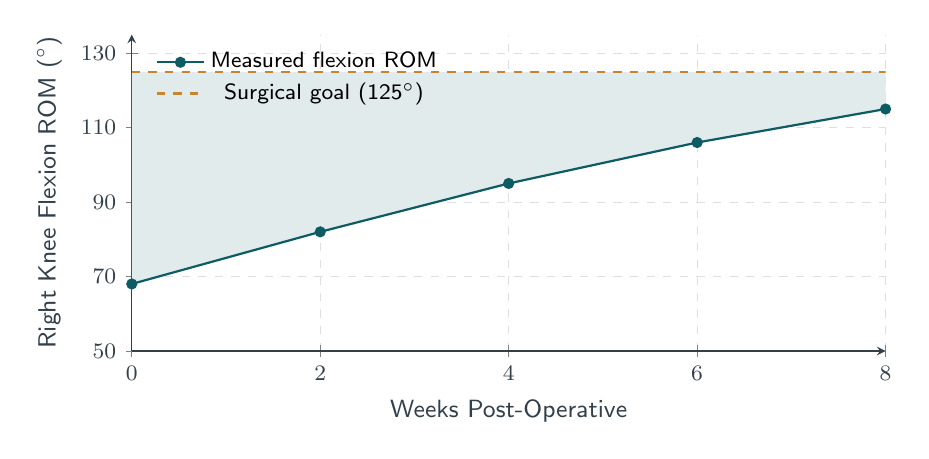
\begin{tikzpicture}
\begin{axis}[
  width=0.92\linewidth,
  height=5.6cm,
  xlabel={\small Weeks Post-Operative},
  ylabel={\small Right Knee Flexion ROM ($^\circ$)},
  xlabel style={font=\sffamily\small,text=ptslate},
  ylabel style={font=\sffamily\small,text=ptslate},
  ymin=50, ymax=135,
  xmin=0, xmax=8,
  xtick={0,2,4,6,8},
  ytick={50,70,90,110,130},
  grid=major,
  grid style={dashed,gray!25},
  axis lines=left,
  axis line style={ptslate},
  tick label style={font=\footnotesize,text=ptslate},
  legend style={font=\footnotesize,draw=none,fill=none,at={(0.02,0.98)},anchor=north west},
]
\addplot[name path=romline,color=ptteal,thick,mark=*,mark options={fill=ptteal,scale=0.8}]
  coordinates {(0,68) (2,82) (4,95) (6,106) (8,115)};
\addlegendentry{Measured flexion ROM}
\addplot[color=ptamber,thick,dashed,mark=none] coordinates {(0,125) (8,125)};
\addlegendentry{Surgical goal (125$^\circ$)}
\addplot[name path=goalline,draw=none,mark=none] coordinates {(0,125) (8,125)};
\addplot[ptteal!12] fill between[of=romline and goalline];
\end{axis}
\end{tikzpicture}
\end{center}
{\footnotesize\color{ptslate}\textit{Figure 1.} Right knee active flexion ROM trend across the current episode of care, plotted against the surgeon-specified functional goal of 125$^\circ$ by discharge.}

% ------------------------------------------------------------------
% ASSESSMENT
% ------------------------------------------------------------------
\sectiontitle{\faClipboard}{Clinical Assessment}

Mr.\ Delgado demonstrates significant, consistent gains in right knee ROM, quadriceps and hip abductor strength, and functional mobility across the eight-week episode, tracking ahead of the typical recovery trajectory for uncomplicated primary TKA. LEFS improvement of 35 points substantially exceeds the minimal clinically important difference. Remaining impairments --- terminal flexion range, stair descent control, and single-leg stance endurance --- are consistent with expected residual deficits at this post-operative interval and are appropriate targets for the next phase of care.

\begin{tcolorbox}[colback=ptbg,colframe=ptgreen,boxrule=0.6pt,arc=1.5pt,
  title={Rehabilitation Potential},fonttitle=\bfseries\sffamily\small,coltitle=white,
  colbacktitle=ptgreen,left=6pt,right=6pt,top=3pt,bottom=3pt]
\small \textbf{Good to Excellent.} Patient is highly motivated, adherent to the home exercise program (self-reported 6/7 days weekly), and free of comorbidities that would limit continued progress. Anticipate discharge to an independent maintenance program by Week 14--16.
\end{tcolorbox}

\vspace{4pt}
% ------------------------------------------------------------------
% GOALS
% ------------------------------------------------------------------
\sectiontitle{\faCheckCircle}{Goals}

\noindent
\begin{minipage}[t]{0.485\linewidth}
\begin{tcolorbox}[goalbox,title={Short-Term Goals (Week 10)}]
\small
\begin{itemize}[leftmargin=14pt,itemsep=3pt,topsep=2pt,label={}]
  \item \metgoal\ Achieve 120$^\circ$ right knee flexion --- \textbf{on track, 115$^\circ$ achieved}
  \item \metgoal\ Full active extension (0$^\circ$) --- \textbf{met}
  \item \opengoal\ Quadriceps MMT 4/5 without extensor lag
  \item \opengoal\ Descend stairs step-over-step without rail
  \item \opengoal\ TUG $<$8.0 seconds
\end{itemize}
\end{tcolorbox}
\end{minipage}\hfill
\begin{minipage}[t]{0.485\linewidth}
\begin{tcolorbox}[goalbox,title={Long-Term Goals (Week 16, Discharge)}]
\small
\begin{itemize}[leftmargin=14pt,itemsep=3pt,topsep=2pt,label={}]
  \item \opengoal\ Achieve 125$^\circ$ right knee flexion, symmetric to left
  \item \opengoal\ Return to unrestricted community ambulation, no device
  \item \opengoal\ Single-leg stance $>$30 seconds bilaterally
  \item \opengoal\ Independent with full home exercise maintenance program
  \item \opengoal\ Clearance to resume recreational doubles tennis
\end{itemize}
\end{tcolorbox}
\end{minipage}
\par

% ------------------------------------------------------------------
% PLAN
% ------------------------------------------------------------------
\sectiontitle{\faCalendar}{Treatment Plan}

\textbf{\color{ptslate}Interventions Performed This Visit}

\begin{tabularx}{\linewidth}{@{}>{\bfseries\raggedright\arraybackslash}p{4.2cm} X@{}}
\toprule
Therapeutic exercise & Closed-chain quadriceps sets, mini-squats to 70$^\circ$, step-ups (15\,cm), standing hip abduction with resistance band, seated terminal knee extension. 3 sets $\times$ 12 reps. \\
Manual therapy & Patellar mobilization grade III, soft tissue mobilization to quadriceps and IT band, joint mobilization for terminal extension. \\
Neuromuscular re-education & Single-leg balance training on foam surface, tandem stance with perturbation, stair descent drilling with visual cueing. \\
Modalities & Cryotherapy 15 minutes post-treatment for effusion management. \\
Patient education & Reviewed progression of home exercise program; instructed in self-mobilization technique for terminal flexion. \\
\bottomrule
\end{tabularx}

\vspace{6pt}
\textbf{\color{ptslate}Plan for Continued Care}

\begin{itemize}[leftmargin=16pt,itemsep=1pt,topsep=2pt]
  \item Continue skilled physical therapy 3x/week for 4 additional weeks, then re-evaluate and transition to 2x/week as goals are met.
  \item Progress closed-chain strengthening load and introduce eccentric step-down training for stair control.
  \item Advance balance program to unstable surfaces and dual-task conditions.
  \item Begin sport-specific lateral agility drills at Week 10 pending surgeon clearance.
  \item Re-evaluate formally at Week 12 with repeat goniometry, MMT, and LEFS administration.
  \item Communicate progress summary to Dr.\ Whitfield prior to the Week 10 post-operative follow-up visit.
\end{itemize}

\vspace{10pt}
\noindent
\begin{tabularx}{\linewidth}{@{}X X@{}}
\rule{5.4cm}{0.4pt} & \rule{5.4cm}{0.4pt} \\
Rachel Nakamura, PT, DPT, OCS \newline Licensed Physical Therapist, OH \#PT-041882 & Date Signed: June 30, 2026 \\
\end{tabularx}

\vspace{4pt}
{\footnotesize\color{ptslate}\textit{Electronically signed and stored in the Meridian Rehabilitation \& Sports Medicine electronic medical record. A copy has been transmitted to the referring physician, Dr.\ Elena Whitfield, Apex Orthopedic Group.}}

\end{document}
